\documentclass{article}[18pt]
\ProvidesPackage{format}
%Page setup
\usepackage[utf8]{inputenc}
\usepackage[margin=0.7in]{geometry}
\usepackage{parselines} 
\usepackage[english]{babel}
\usepackage{fancyhdr}
\usepackage{titlesec}
\hyphenpenalty=10000

\pagestyle{fancy}
\fancyhf{}
\rhead{Sam Robbins}
\rfoot{Page \thepage}

%Characters
\usepackage{amsmath}
\usepackage{amssymb}
\usepackage{gensymb}
\newcommand{\R}{\mathbb{R}}

%Diagrams
\usepackage{pgfplots}
\usepackage{graphicx}
\usepackage{tabularx}
\usepackage{relsize}
\pgfplotsset{width=10cm,compat=1.9}
\usepackage{float}

%Length Setting
\titlespacing\section{0pt}{14pt plus 4pt minus 2pt}{0pt plus 2pt minus 2pt}
\newlength\tindent
\setlength{\tindent}{\parindent}
\setlength{\parindent}{0pt}
\renewcommand{\indent}{\hspace*{\tindent}}

%Programming Font
\usepackage{courier}
\usepackage{listings}
\usepackage{pxfonts}

%Lists
\usepackage{enumerate}
\usepackage{enumitem}

% Networks Macro
\usepackage{tikz}


% Commands for files converted using pandoc
\providecommand{\tightlist}{%
	\setlength{\itemsep}{0pt}\setlength{\parskip}{0pt}}
\usepackage{hyperref}

% Get nice commands for floor and ceil
\usepackage{mathtools}
\DeclarePairedDelimiter{\ceil}{\lceil}{\rceil}
\DeclarePairedDelimiter{\floor}{\lfloor}{\rfloor}

% Allow itemize to go up to 20 levels deep (just change the number if you need more you madman)
\usepackage{enumitem}
\setlistdepth{20}
\renewlist{itemize}{itemize}{20}

% initially, use dots for all levels
\setlist[itemize]{label=$\cdot$}

% customize the first 3 levels
\setlist[itemize,1]{label=\textbullet}
\setlist[itemize,2]{label=--}
\setlist[itemize,3]{label=*}

% Definition and Important Stuff
% Important stuff
\usepackage[framemethod=TikZ]{mdframed}

\newcounter{theo}[section]\setcounter{theo}{0}
\renewcommand{\thetheo}{\arabic{section}.\arabic{theo}}
\newenvironment{important}[1][]{%
	\refstepcounter{theo}%
	\ifstrempty{#1}%
	{\mdfsetup{%
			frametitle={%
				\tikz[baseline=(current bounding box.east),outer sep=0pt]
				\node[anchor=east,rectangle,fill=red!50]
				{\strut Important};}}
	}%
	{\mdfsetup{%
			frametitle={%
				\tikz[baseline=(current bounding box.east),outer sep=0pt]
				\node[anchor=east,rectangle,fill=red!50]
				{\strut Important:~#1};}}%
	}%
	\mdfsetup{innertopmargin=10pt,linecolor=red!50,%
		linewidth=2pt,topline=true,%
		frametitleaboveskip=\dimexpr-\ht\strutbox\relax
	}
	\begin{mdframed}[]\relax%
		\centering
		}{\end{mdframed}}



\newcounter{lem}[section]\setcounter{lem}{0}
\renewcommand{\thelem}{\arabic{section}.\arabic{lem}}
\newenvironment{defin}[1][]{%
	\refstepcounter{lem}%
	\ifstrempty{#1}%
	{\mdfsetup{%
			frametitle={%
				\tikz[baseline=(current bounding box.east),outer sep=0pt]
				\node[anchor=east,rectangle,fill=blue!20]
				{\strut Definition};}}
	}%
	{\mdfsetup{%
			frametitle={%
				\tikz[baseline=(current bounding box.east),outer sep=0pt]
				\node[anchor=east,rectangle,fill=blue!20]
				{\strut Definition:~#1};}}%
	}%
	\mdfsetup{innertopmargin=10pt,linecolor=blue!20,%
		linewidth=2pt,topline=true,%
		frametitleaboveskip=\dimexpr-\ht\strutbox\relax
	}
	\begin{mdframed}[]\relax%
		\centering
		}{\end{mdframed}}
\lhead{Software Engineering}


\begin{document}
\begin{center}
\underline{\huge What is Software Engineering?}
\end{center} 
\section{ISP - Ill-structured problems}
\begin{itemize}
	\item Many possible solutions, good/bad rather than right/wrong
	\item No definitive test of any outcome
	\item No 'stopping rule' that can be used to determine that a solution (or an optimum one) has been reached
	\item No definitive formulation. Our understanding of the nature of the problem is entwined with our ideas about solving it
\end{itemize}
\begin{center}
	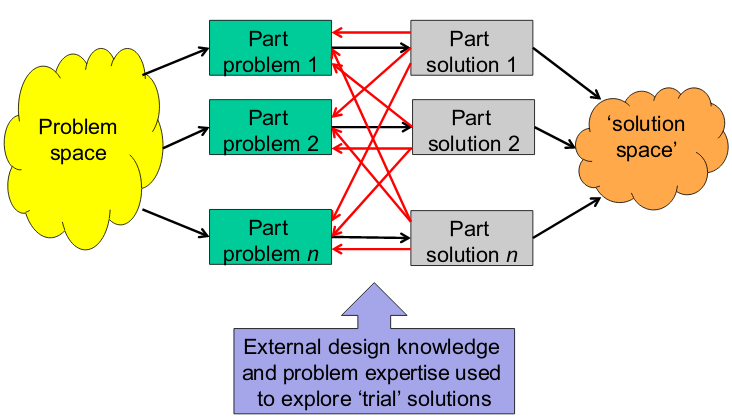
\includegraphics[scale=0.7]{ISP}
\end{center}
\subsection{Addressing an ISP}
Learning how to address ISPs requires you to learn effective ways to explore ideas (rather than learning the 'right' way to do something)
\section{WSP - Well-structured problems}
\begin{itemize}
	\item The existence of a 'right' solution/answer
	\item Having a specific criterion for testing any proposed solution
	\item Having at least one problem space in which the initial problem state, goal state, and all other states that may be reached, can be represented
\end{itemize}
\begin{center}
	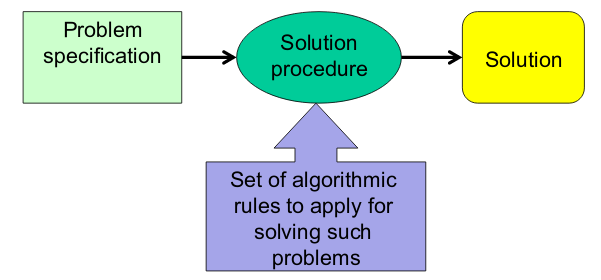
\includegraphics[scale=0.7]{Solve}
\end{center}
\section{Software Development}
\begin{itemize}
	\item Computer programming is an example of an ISP. Even on a small scale, different people produce quite individual programs to meet a specific need
	\item So, more or less anything related to 'programming in the large' (software development) is going to be concerned with ISPs. Which means that SE will be largely concerned with 'solving' ISPs
\end{itemize}
\subsection{What is SE about?}
Early thinking about how to do this sought to mix design concepts with formal and rigorous ideas drawn from science.  However, as understanding has evolved it has become recognised that there is a strong element of social process involved too, and that human factors play a major role in the various activities.
\section{Technical Debt}
\begin{itemize}
	\item Decisions in many software engineering activities will involve making trade-offs between different characteristics of a solution (design)
	\item A term often used in SE for a major form of trade-off is technical debt. This reflects the implied cost that additional later reworking of the system will impose if we choose an easy solution now, instead of going for a better solution that will take longer.
	\item This reflects a key difference of perspective related to software development: students rarely rework code; whereas in industry, it occurs extensively.
\end{itemize}
\section{How ISP characteristics affect (exam) assessment}
\begin{center}
	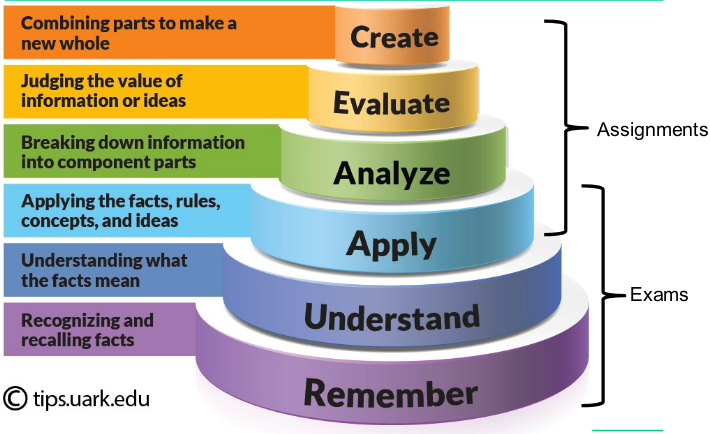
\includegraphics[scale=0.7]{Bloom}
\end{center}
\subsection{Exam words}
\textbf{Remembering} - Distinguished by words such as 'describe'\\
\textbf{Understanding} - Needs to be demonstrated for 'explain'\\
\textbf{Application} - Involves some form of problem.
\section{Design rather than scientific analysis}
\subsection{What do we mean by design}
\textbf{Product} - Related to styling\\
\textbf{Planning} - Use familiar items, layouts\\
\textbf{Engineering} - Adapting past experience and domain knowledge to create a new way of doing something
\subsection{Software Engineering}
\begin{itemize}
	\item A 'construction and use' perspective on computing
	\item Major knowledge elements include:
	\begin{itemize}
		\item Systems/software concepts and strategies
		\item Systems/software management
		\item Computer concepts
	\end{itemize}
	\item Knowledge is largely encapsulated as 'lessons' from experience (plan-driven methods) or in the form of models (such as diagrams)
	\item Research largely uses non-mathematical forms of analysis and 'concept implementation'
\end{itemize}
\subsection{Example: Developing a Web Browser}
\begin{itemize}
	\item CS: Algorithms for finding pages, ways of formatting pages
	\item SE: Structuring of browser objects, development planning, coding, testing
	\item IS (Information Systems): What end users might use it for, how they organise the way they use it in order to meet their needs
\end{itemize}
Remember that design thinking applies to many of the activities that occur on software development, not just to 'system design'
\section{Characteristics and Challenges}
\begin{itemize}
	\item Abstraction
	\item Static vs Dynamic properties
	\item Complexities
	\item Quantity measures
	\item (no) Manufacturing cycle
	\item Evolution
	\item People issues
\end{itemize}
\section{Why Software Engineering Matters}
\begin{center}
	\includegraphics[scale=0.7]{"Hype Cycle"}
\end{center}






\end{document}